\documentclass[preprint,acmtog]{acmart}

\usepackage[utf8]{inputenc}
\usepackage{booktabs} % For formal tables
\usepackage{mathtools}

\graphicspath{{img/}{build/}{./}}

% \acmPrice{0.00}

% The next eight lines come directly from the completed rights form.
% You MUST replace them with the lines specific to your accepted work.
% \setcopyright{acmlicensed}
% \acmJournal{TOG}
% \acmYear{2017}
% \acmVolume{36}
% \acmNumber{4}
% \acmArticle{1}
% \acmMonth{7}
% \acmDOI{http://dx.doi.org/10.1145/8888888.7777777}

% Use the "authoryear" citation style, and make sure citations are in [square brackets].
\citestyle{acmauthoryear}
\setcitestyle{square}
\setcopyright{none}

% A useful command for controlling the number of authors per row.
% The default value of "authorsperrow" is 2.
\settopmatter{authorsperrow=4}

% end of preamble.

\begin{document}

% Title.
% If your title is long, consider \title[short title]{full title} - "short title" will be used for running heads.
\title{Autonomous Calibration of 3D Computer Vision System}

% Authors.
\author{Gustaf Waldemarson}
\affiliation{%
  \institution{Lund University},
  \institution{Arm Sweden AB}}
\email{gustaf.waldemarson@arm.com}

\author{Martin Larsson}
\affiliation{%
  \institution{Lund University}}
\email{martin.larsson@math.lth.se}

\author{Olivier Moliner}
\affiliation{%
  \institution{Lund University},
  \institution{Sony}}
\email{olivier.moliner@sony.com}

\author{Lissy Pellaco}
\affiliation{%
  \institution{KTH Royal Institute of Technology}}
\email{pellaco@kth.se}

\author{Xuechun Xu}
\affiliation{%
  \institution{KTH Royal Institute of Technology}}
\email{chunx@kth.se}

\author{Håkan Carlsson}
\affiliation{%
  \institution{KTH Royal Institute of Technology}}
\email{hakcar@kth.se}

\author{Mina Ferizbegovic}
\affiliation{%
  \institution{KTH Royal Institute of Technology}}
\email{minafe@kth.se}

% This command defines the author string for running heads.
\renewcommand{\shortauthors}{Waldemarson, Larsson, Moliner, Pellaco, Xu, Carlsson, Ferizbegovic}

% abstract
\begin{abstract}
  Cameras are often useful for a wide variety of tasks in autonomous systems and
  with two or more, it is possible to reason about the scene in 3D from each
  image. However, in order to use the cameras in this way, they must be
  calibrated beforehand using objects with known geometries. This requires
  several manual steps that must be repeated each time the internal camera
  parameters change.

  This report investigates methods and techniques that can be used to remove
  this limitation: Using IMU data, the relative positions and orientation of an
  array of three or more cameras can be estimated and passed on to a vision
  system for automatically compute the intrinsic camera parameters with minimal
  or no prior knowledge of the scene. Effectively calibrating the cameras
  without user intervention.
\end{abstract}

% CCS
\begin{CCSXML}
  <ccs2012>
  <concept>
  <concept_id>10010147.10010178.10010224.10010226.10010234</concept_id>
  <concept_desc>Computing methodologies~Camera calibration</concept_desc>
  <concept_significance>500</concept_significance>
  </concept>
  </ccs2012>
\end{CCSXML}

\ccsdesc[500]{Computing methodologies~Camera calibration}

% keywords
\keywords{camera calibration, multiple views, IMU, Scene Reconstruction}

% A "teaser" figure, centered below the title and authors and above the body of the work.
\begin{teaserfigure}
  \centering
  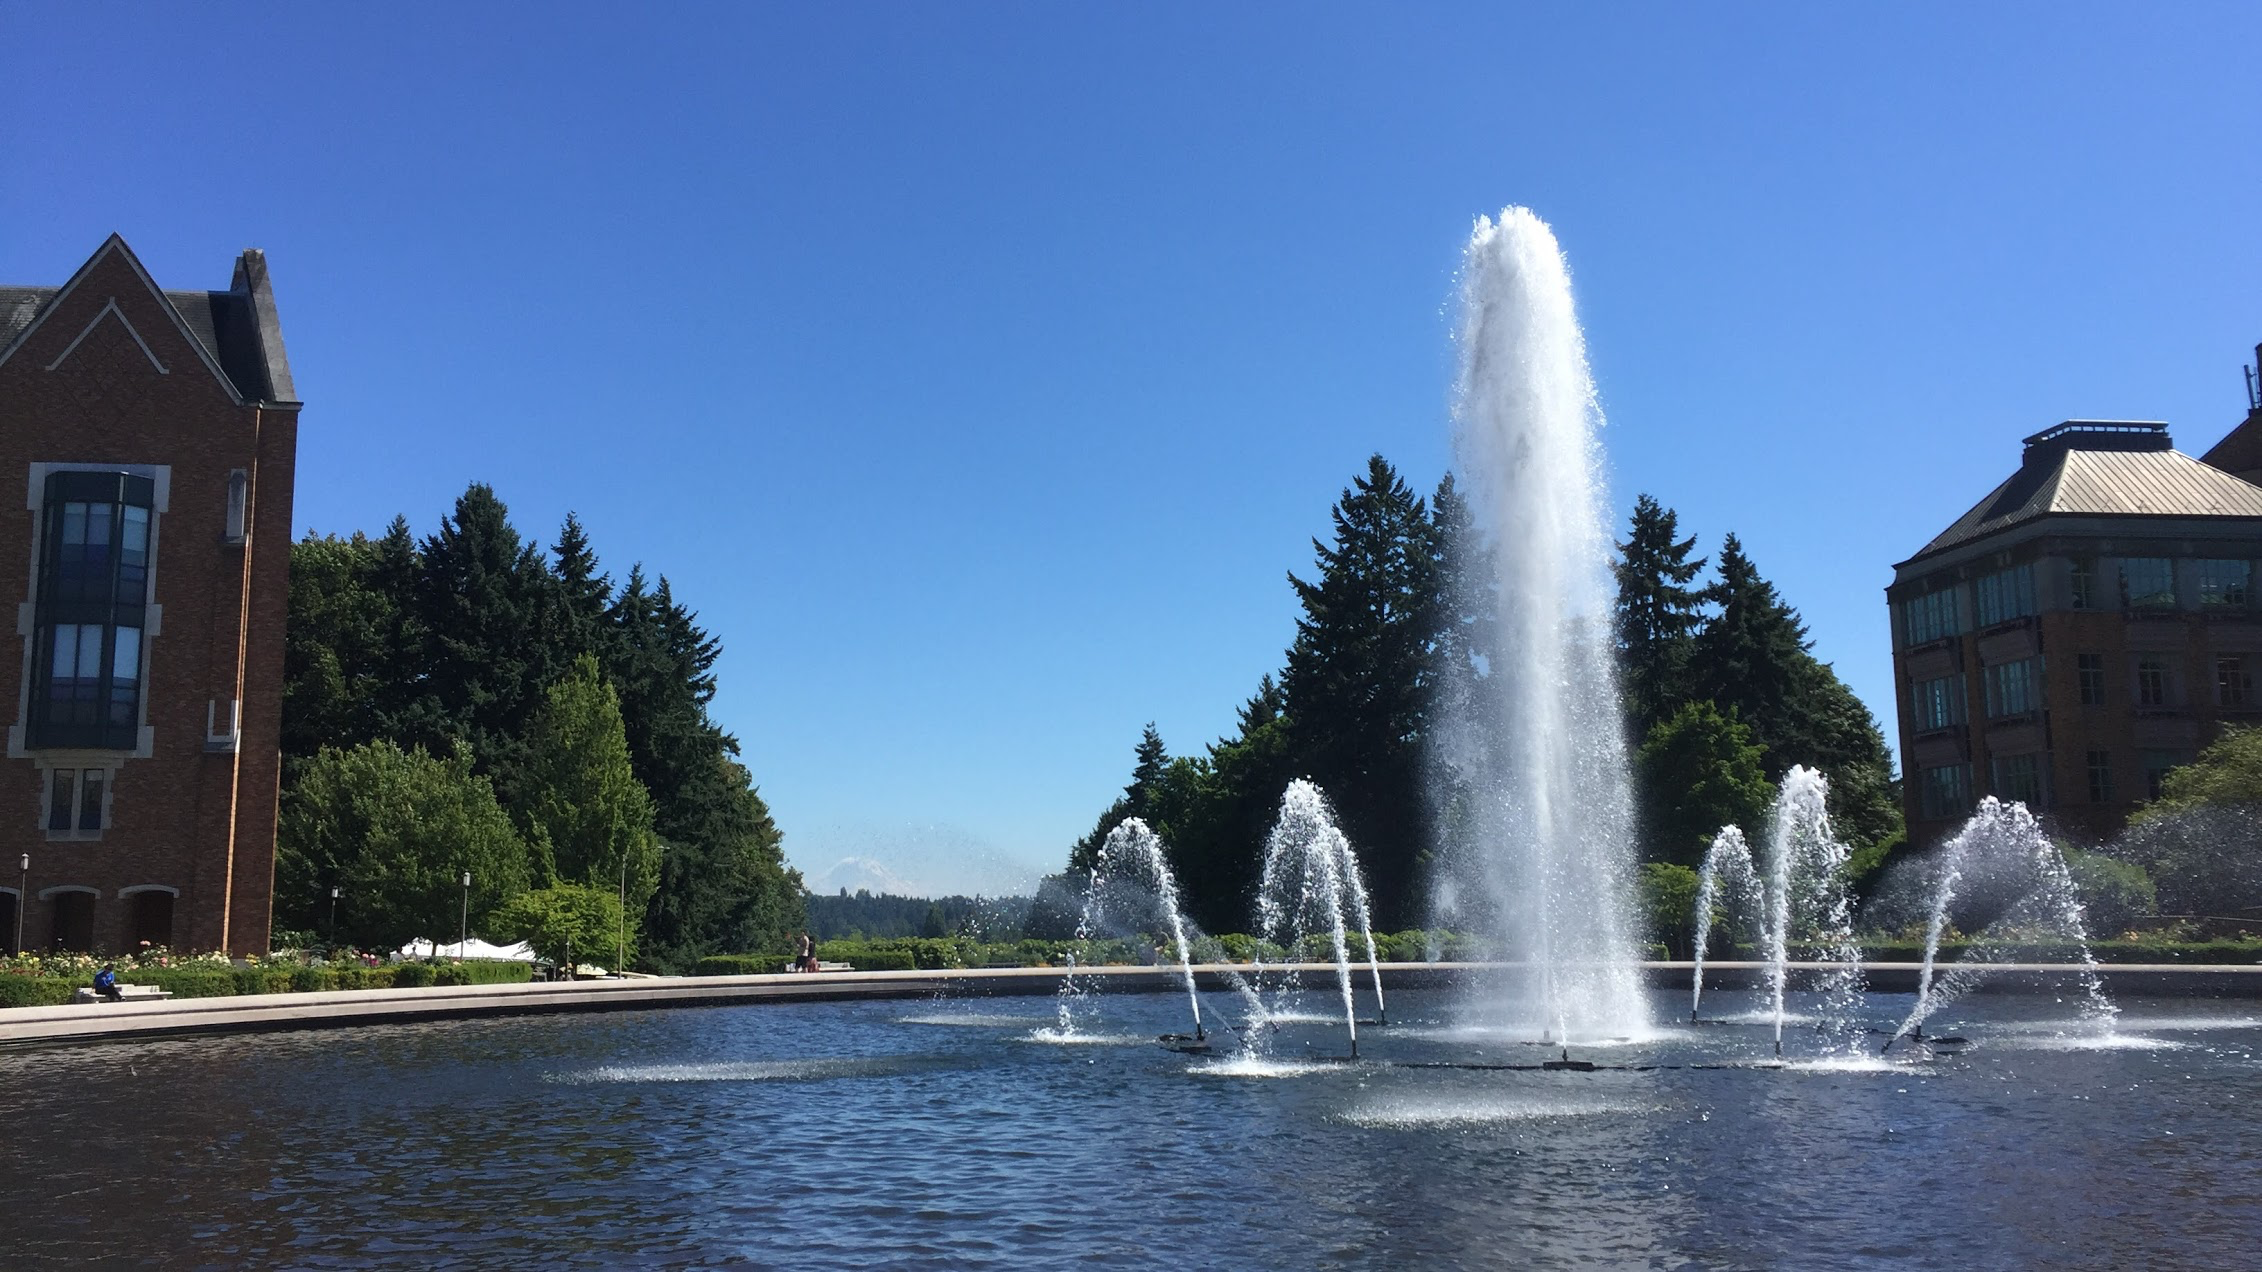
\includegraphics[width=6.0in]{fountain}
  \caption{Drumheller Fountain, The University of Washington, Seattle WA.}
\end{teaserfigure}

% Processes all of the front-end information and starts the body of the work.
\maketitle

\section{Introduction}

% TODO: IMU introduction merge.

Cameras are an important component in many systems. And modern cameras are often
equipped with additional features, such as varifocal lenses to allow them to
adjust and zoom into various parts of any given scene. In order to use these
cameras in larger systems, they must often be manually calibrated before
use. This also means that the zooming features described above become
unavailable, as changing the zoom would change the intrinsic parameters of the
camera and would invalidate the calibration.

For this reason, it is desirable to have a system that can automatically
calibrate itself, preferably without prior knowledge scene it will be working
inside.


\subsection{The Correspondence Problem}



\section{Related Work}

% TODO: Related work in regard to the IMU calibration.

The problem presented in this report is most similar to the problem presented by
Bundler~\cite{bundler2006}. That is, using an unstructured collection of images
estimate the 3D structure of the scene as well as both the intrinsic and
extrinsic camera parameters. The primary difference in this case is that by
using the known relative position and orientation of the cameras as provided
beforehand or by IMUs, we are able to significantly simplify the problem and
make it easier to calibrate the cameras with limited scene structure or limited
variation in camera poses inside the scene.

% TODO: Create image to show this. I.e., all cameras primarily from one side, as
% opposed to everywhere around it as in the case of bundler.

\section{Method}

\subsection{IMU Calibration}

\subsection{Camera Calibration}

The majority of the vision part of this project uses off the shelf components
and algorithms from e.g., OpenCV~\cite{opencv_library} and
Ceres~\cite{ceres-solver} to solve the various steps involved in this
problem. All of which are described in detail below.

\subsubsection{Feature Detection}

The most important part for making sense of the scene is finding image
coordinates that are representative of some particular property in the
image. Colloquially, these are known as image feature, or feature descriptors.

Feature detection has been an active research topic for many years but in this
paper we settled for using a proven feature detector that is known to not be
patent encumbered. That is, the so called ORB feature detector~\cite{orb2011}.


\subsubsection{Feature Matching}

Once feature points have been found they need to be matched between images in
order to be of further use. This process starts by iterating over all possible
pairs of images and then computes the normalized Hamming distance for each pair
of feature descriptors. After this, several passes of filtering is run to remove
low quality matches. First, the Lowe criteria~\cite{sift2004} is applied,
followed by a RANSAC~\cite{ransac} estimation of the fundamental matrix between
the remaining pairs.

\begin{figure}[ht]
  \centering
  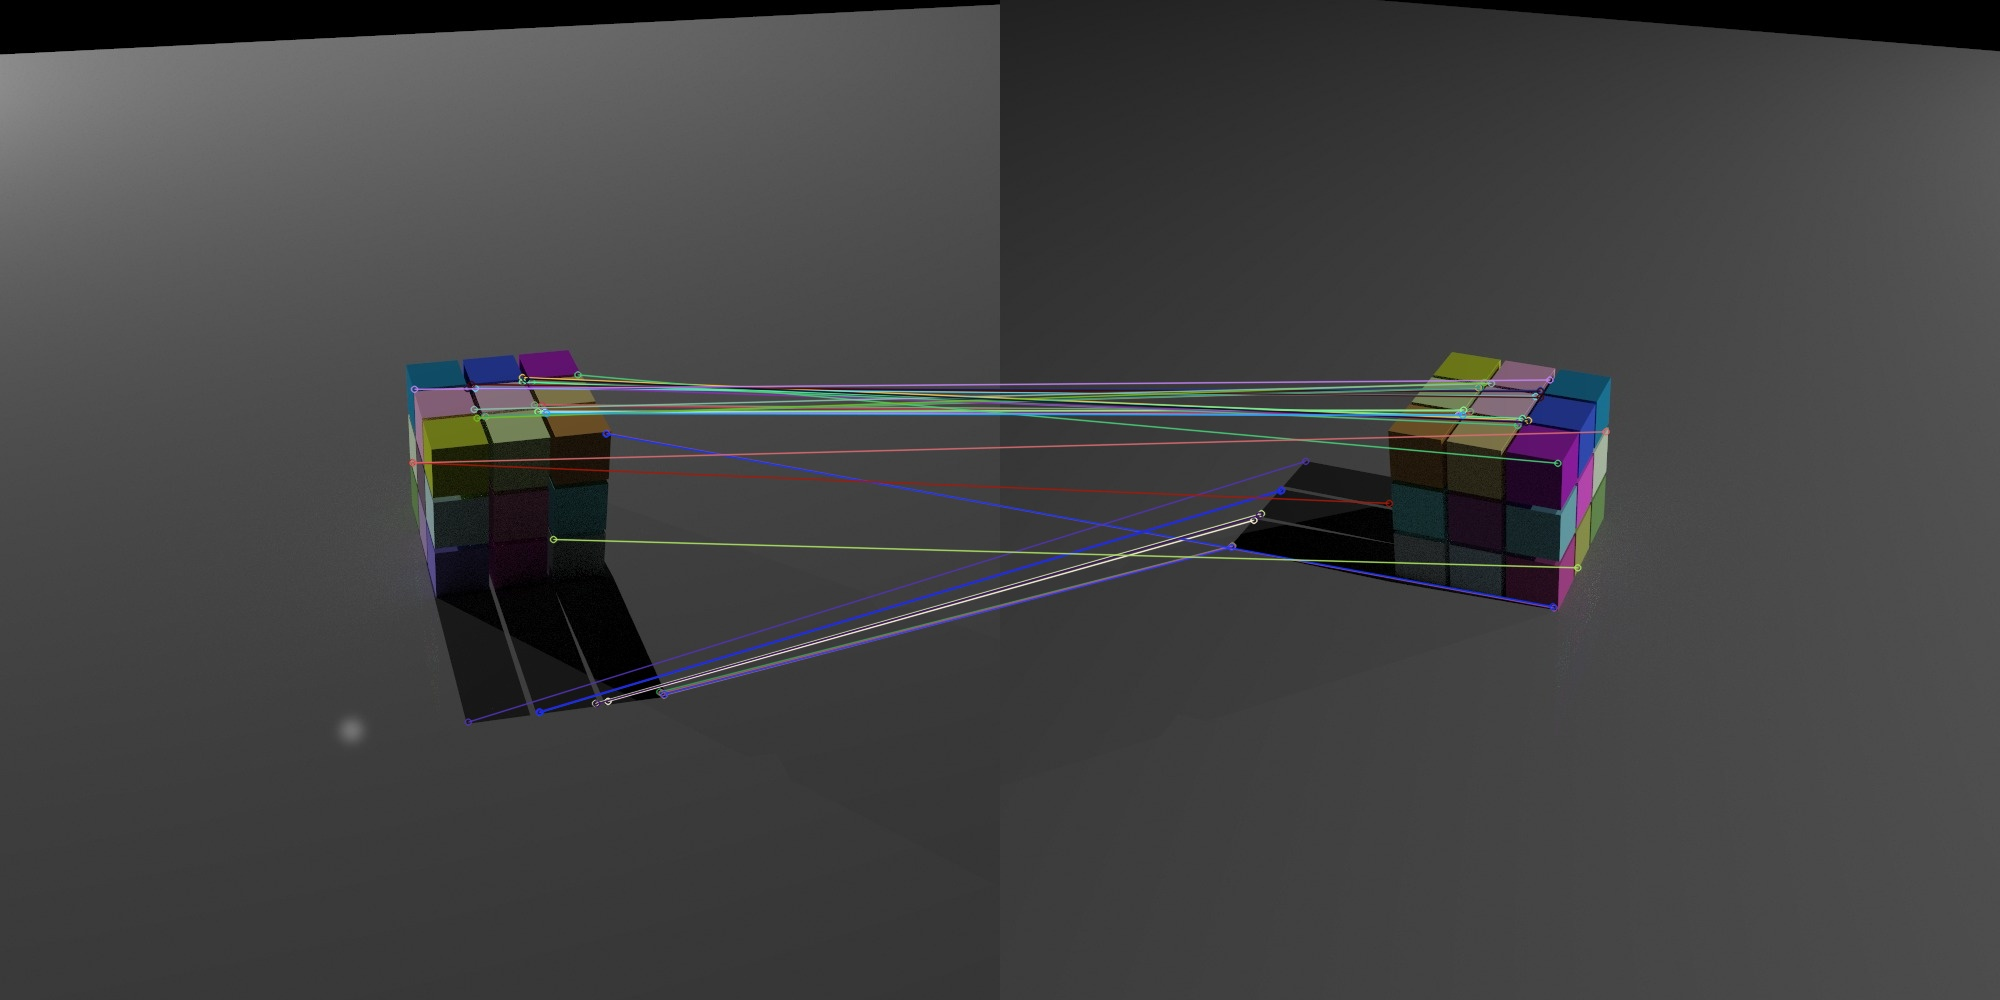
\includegraphics[width=1.0\linewidth]{matches_3}
  \caption{Example from the pairwise feature matching.}
\end{figure}


% TODO: Create pseudo-algorithm describing the matching procedure.

The points that remain are now passed onward in the algorithm, where they will
be filtered against multiple pairs of images.


\subsubsection{Track Detection}

Once all pairs of images have been matched, they are compiled into a graph where
each vertex is an image keypoint and each edge represent a match between
keypoints.

\begin{figure}[ht]
  \centering
  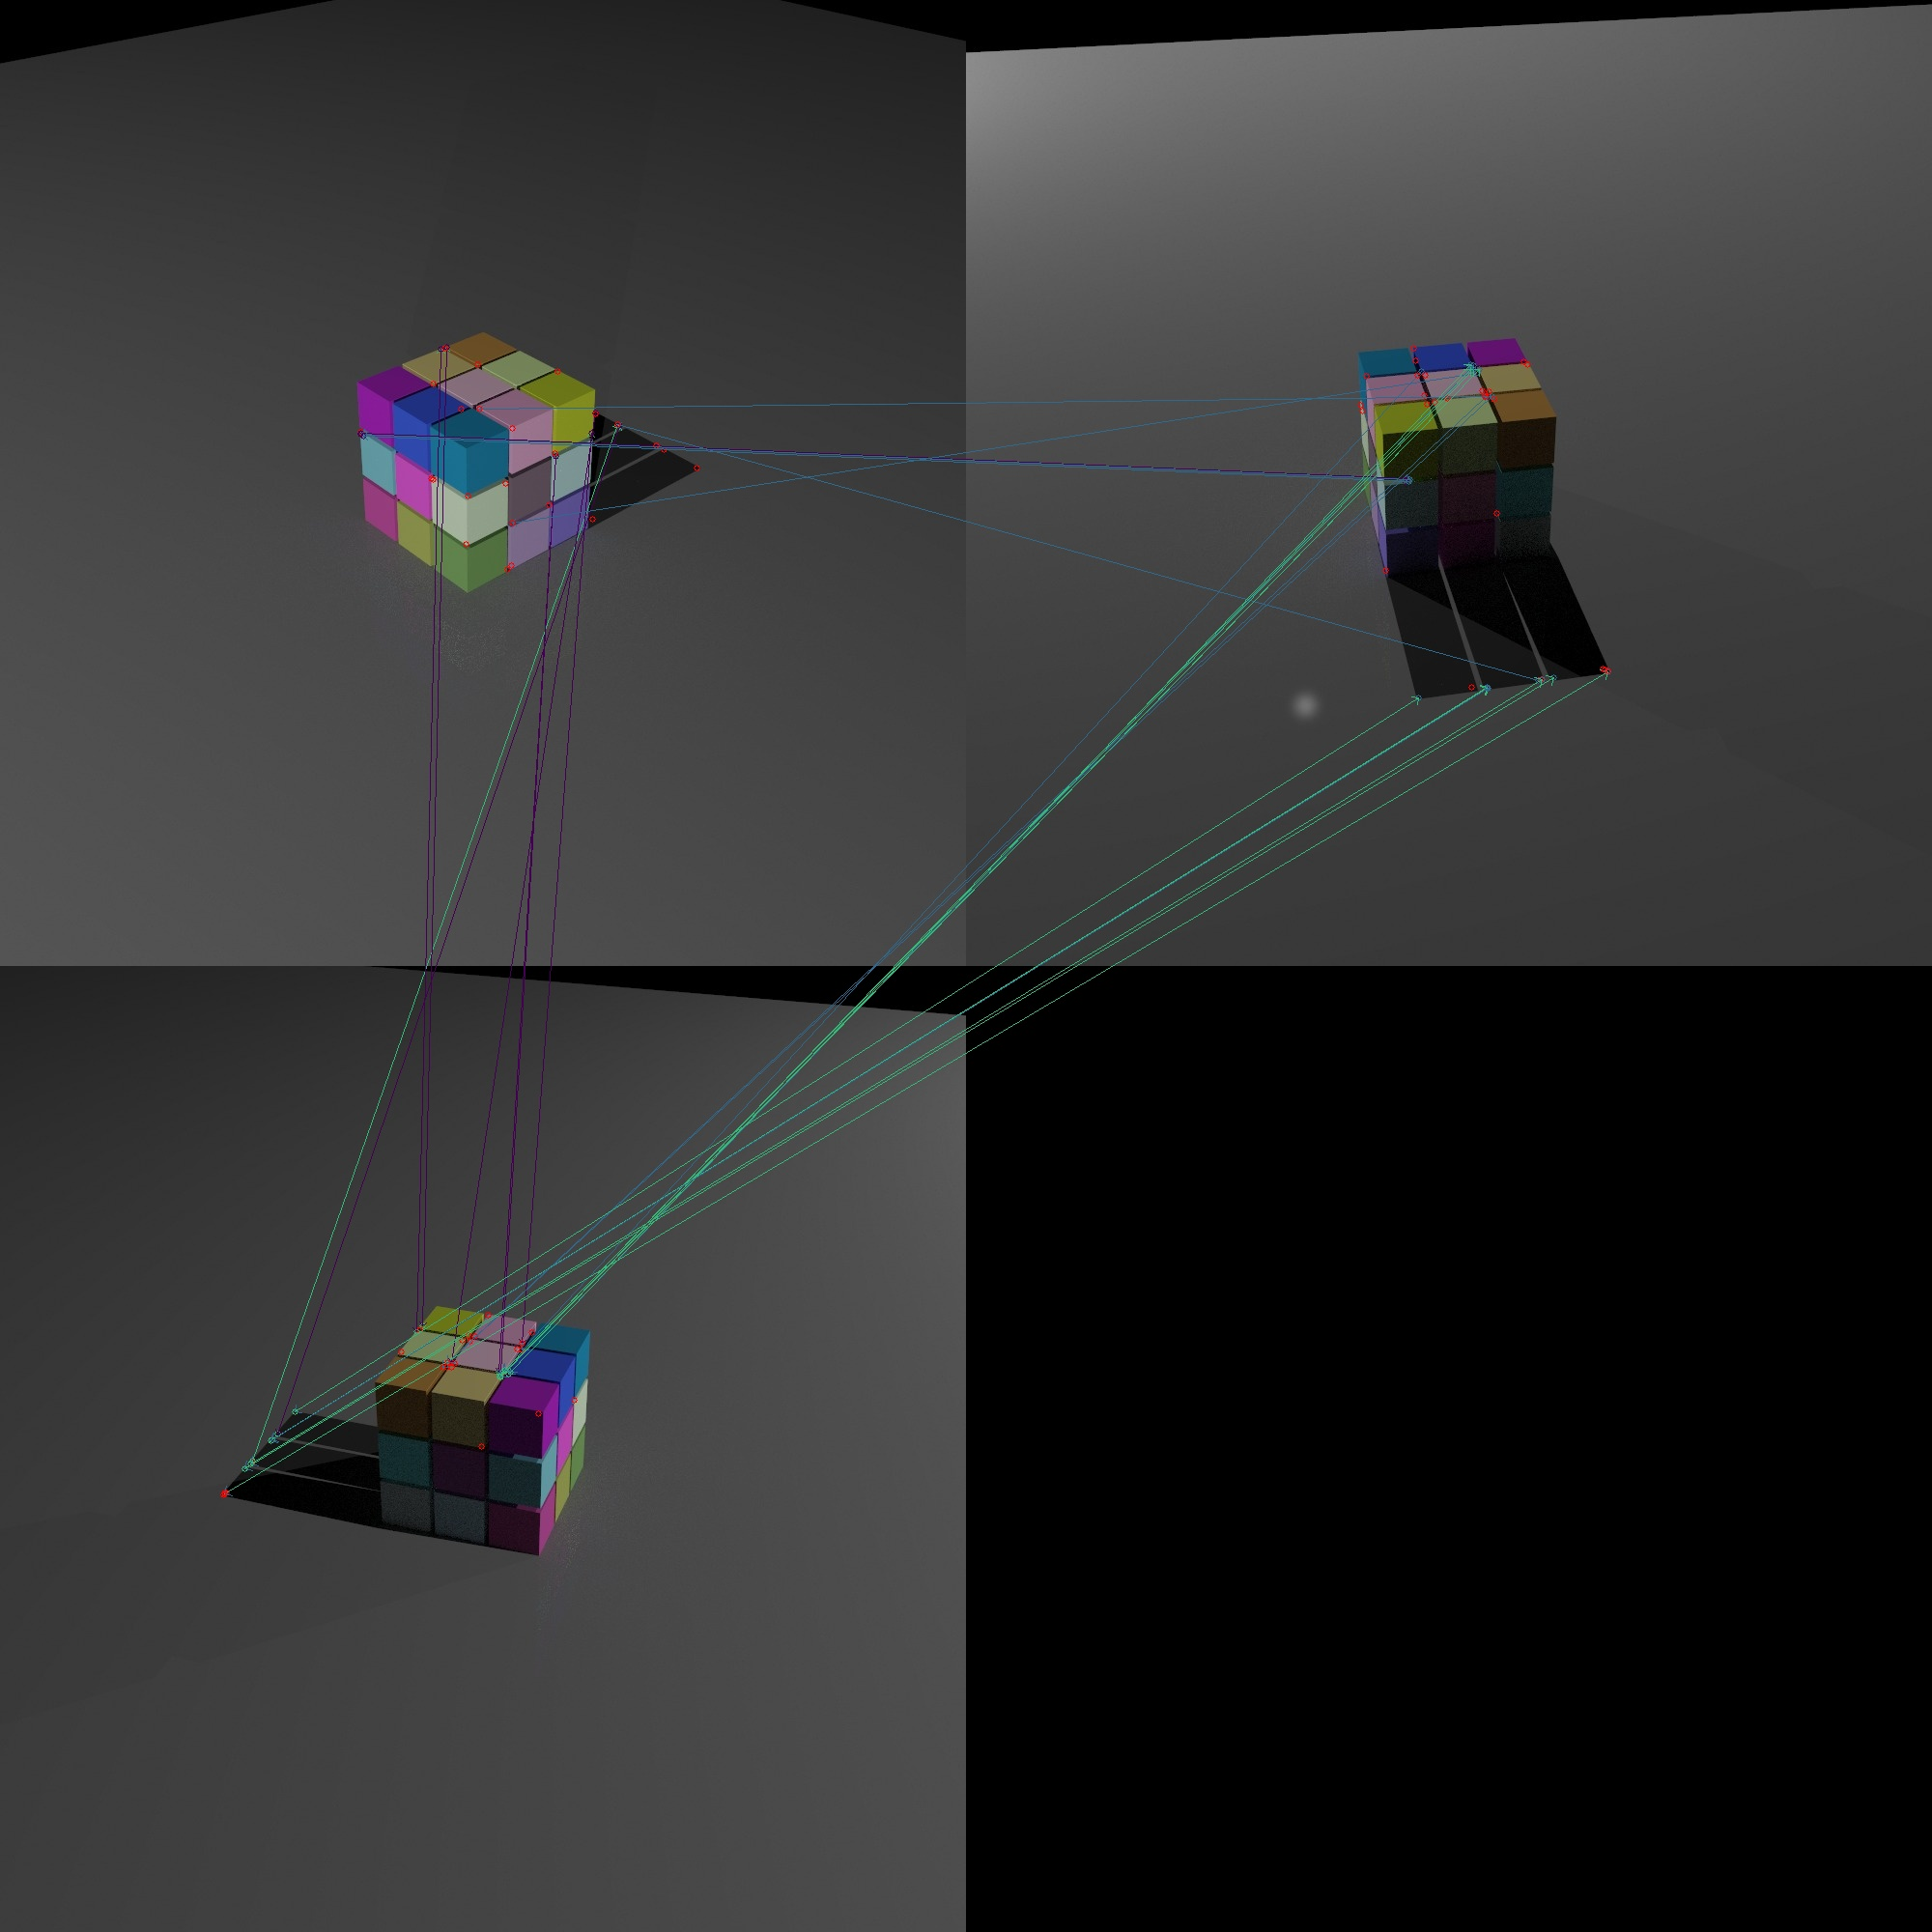
\includegraphics[width=1.0\linewidth]{filtered_image_graph}
  \caption{The image graph: All pairwise matches compiled into a single
    graph. Here displayed on top of the source images. Note that red dots
    represent removed matches.}
\end{figure}

Using graph processing techniques, is possible to use this graph to find
keypoints that are common between multiple pairs of images. These collections of
keypoints are now marked grouped into \emph{tracks}: A structure that represent
a single 3D point that is presumably visible in multiple images.

Additionally, pairs that are commutative i.e., image pair (A, B) finds the same
keypoint as (B, A), are marked during this process, as they are very likely to
correspond to a single 3D point, despite yielding a very small track.


\subsubsection{Bundle Adjustment}

Using the image tracks, the final step of the problem is creating and solving a
non-linear system of equations on the form:
%
\begin{equation*}
  \mathbf{x}_{j} = f(\mathbf{X}_{i})
\end{equation*}
%
where $\mathbf{X}_{i}$ represents a 3D point in the scene and $\mathbf{x}_{j}$
is the projected image point of $\mathbf{X_{i}}$ from camera $j$. Depending on
the chosen camera model, $f(\cdot)$ can be a simple projective pin-hole camera on
the form:
%
\begin{equation*}
  f(\mathbf{X}_{i}) =
  K \begin{bsmallmatrix}R & | & t\end{bsmallmatrix} \mathbf{X}_{i}
\end{equation*}
%
Where $K$ is the intrinsic camera parameter matrix, $R$ is a rotation matrix and
$t$ is a translation vector. Alternatively, $f(\cdot)$ can include rectification to
adjust for a variety of camera distortion, which adds a number of parameters to
the camera model.

All of this is fed into Ceres~\cite{ceres-solver}, which performs
auto-differentiation of the selected camera function to compute the Jacobian
matrix necessary for the final step, which executes the Levenberg-Marquardt
algorithm~\cite{More78}, which ultimately solves our problem; estimating the
intrinsic and extrinsic camera parameters as well as finding 3D coordinates for
some points in the scene.


\section{Results}

In the absence of a rig that would be able to report accurate positions and
images at each time, synthetic images were generated by a 3D rendering
system. For this report, the images in~\ref{fig:camgraph} were used.
%
\begin{figure}
  \label{fig:camgraph}
  \begin{tabular}{ccc}
    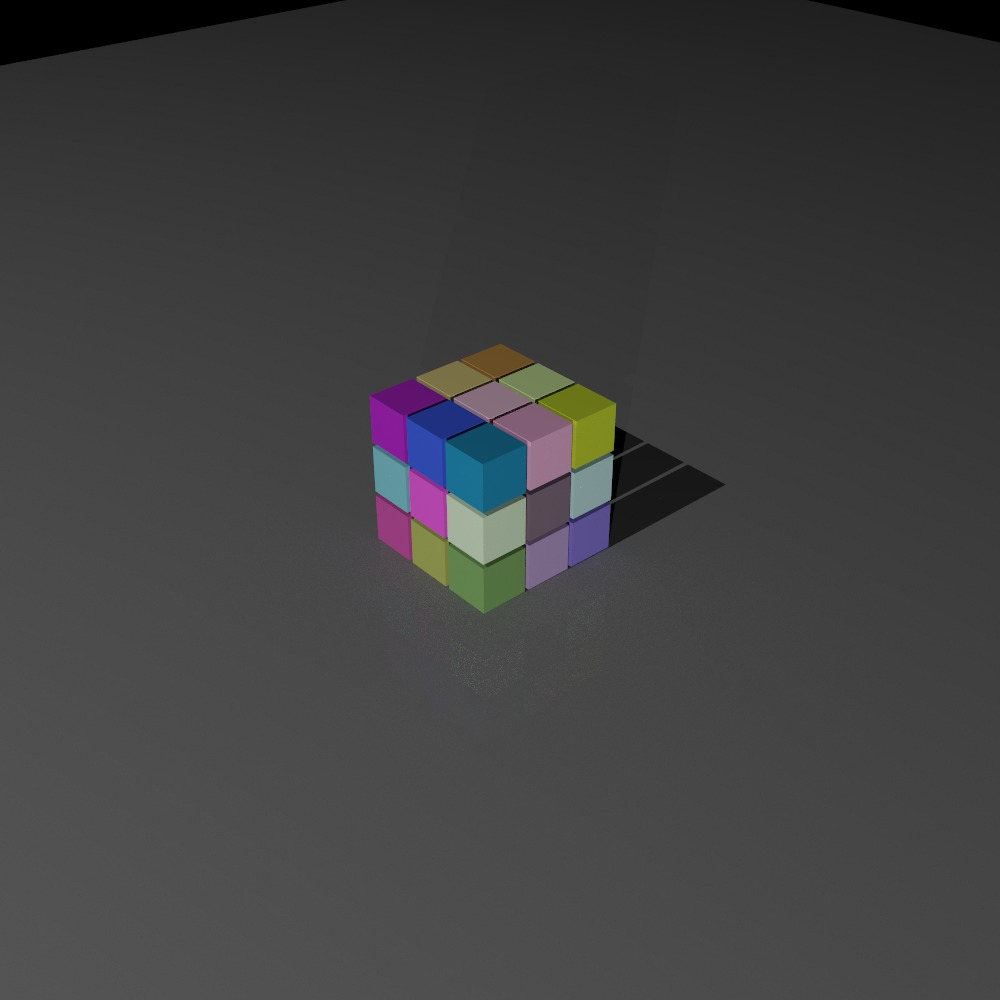
\includegraphics[width=0.3\linewidth]{cam-000} &
    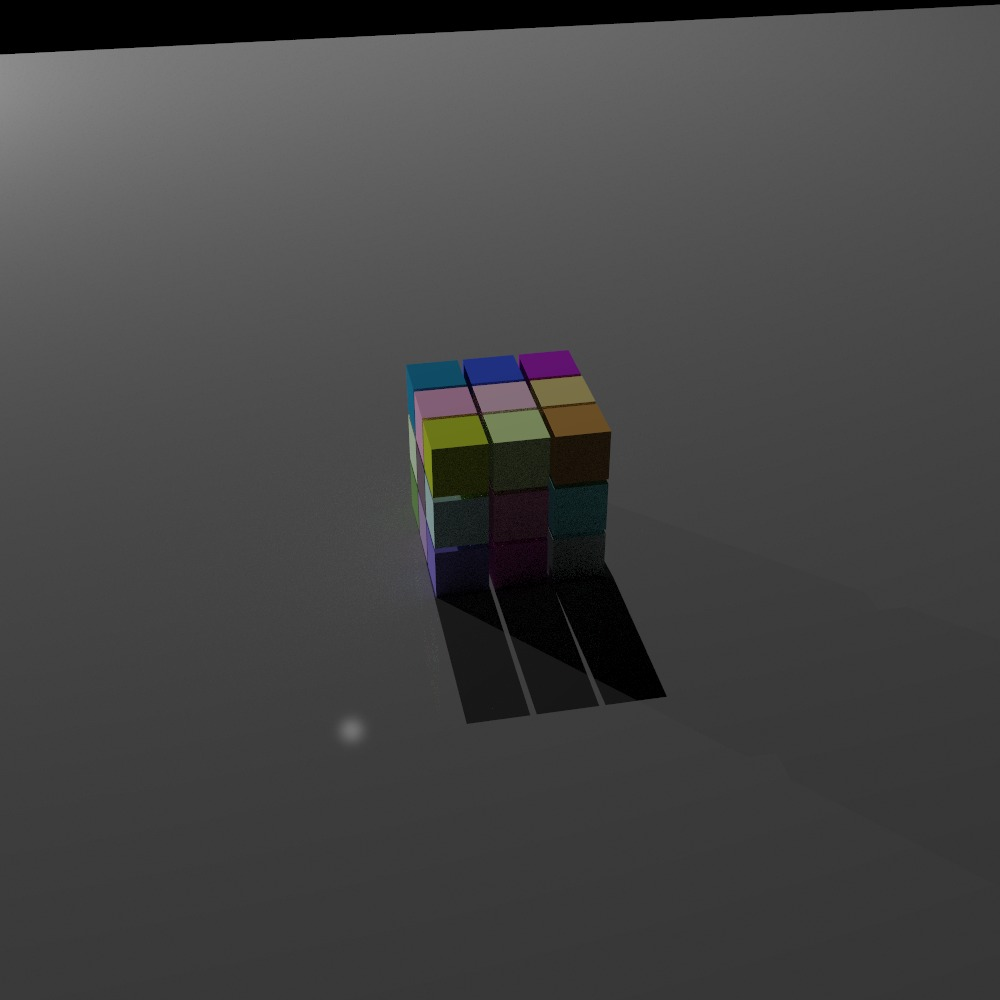
\includegraphics[width=0.3\linewidth]{cam-001} &
    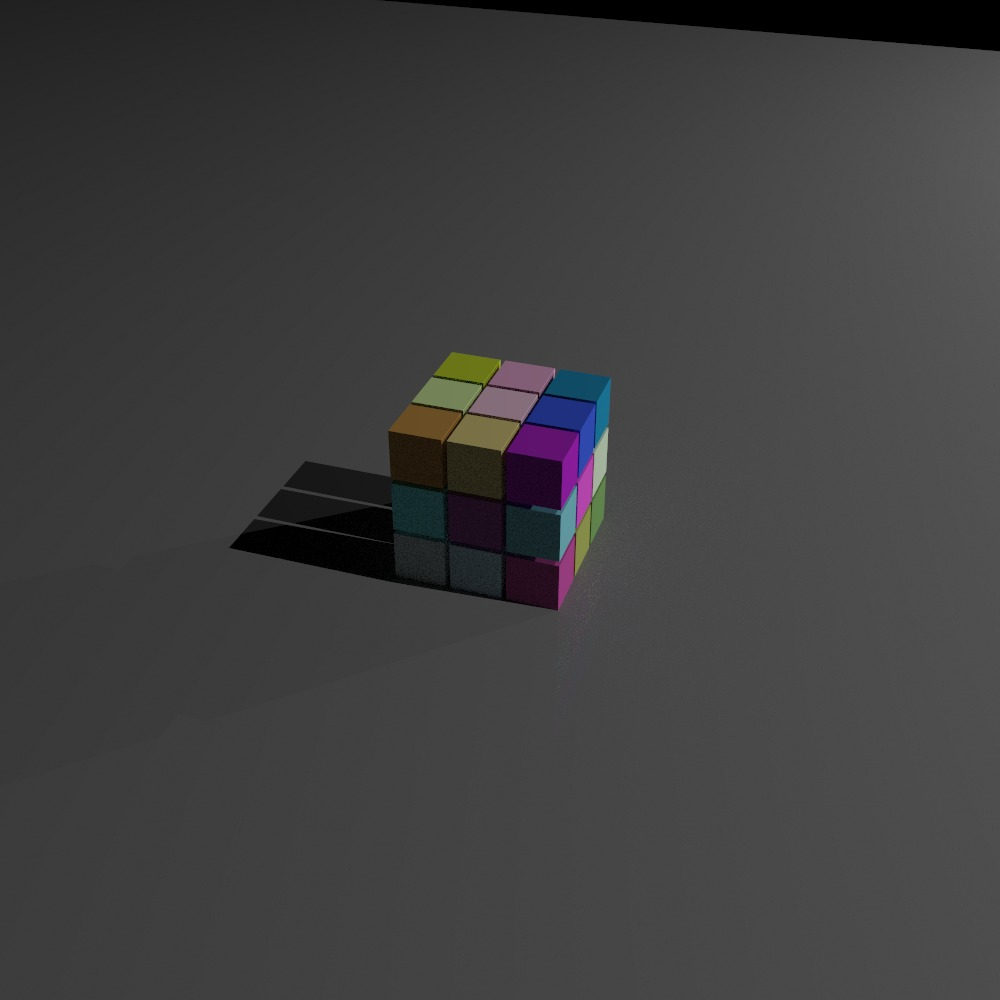
\includegraphics[width=0.3\linewidth]{cam-002}
  \end{tabular}
  \caption{Synthetic images our procedure were trialed on.}
\end{figure}
%
The recovered 3D scene structure can be seen in figure~\ref{fig:sfm}.
%
\begin{figure}
  \label{fig:sfm}
  \begin{tabular}{cc}
    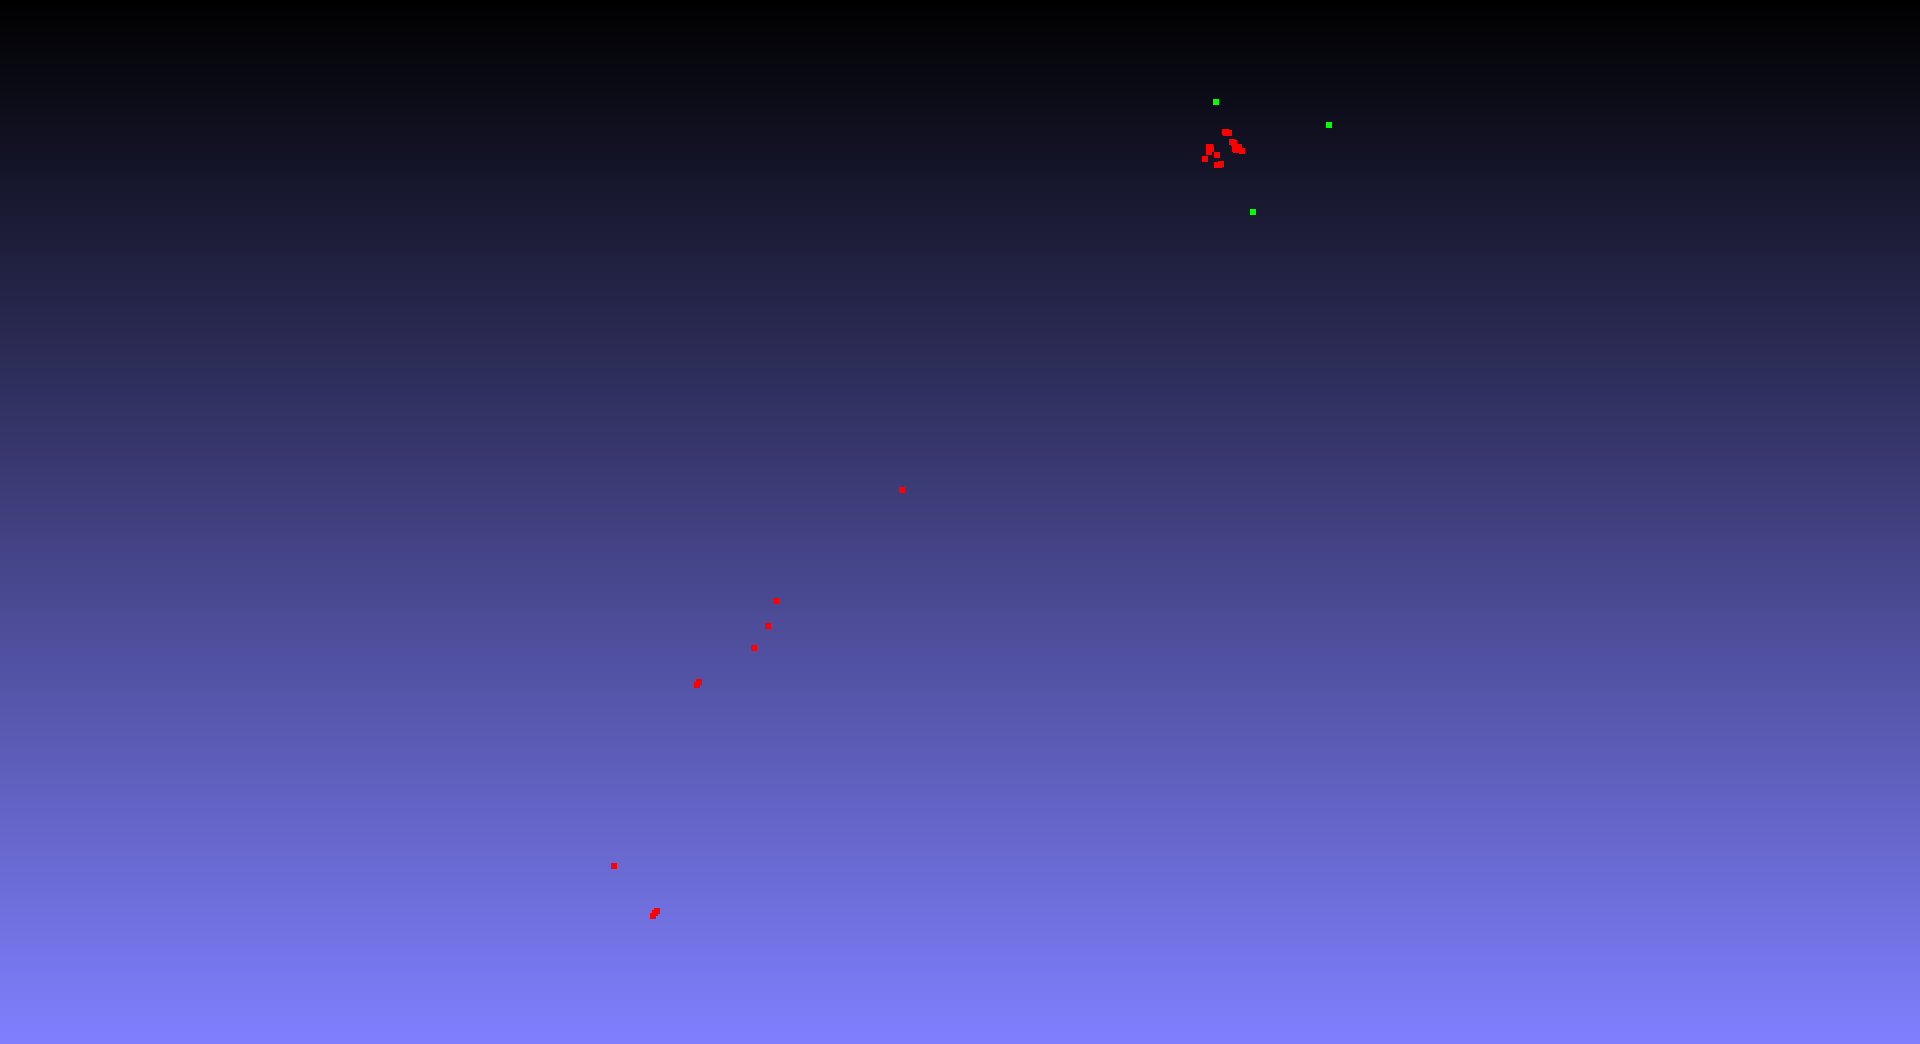
\includegraphics[width=0.5\linewidth]{sfm_all} &
    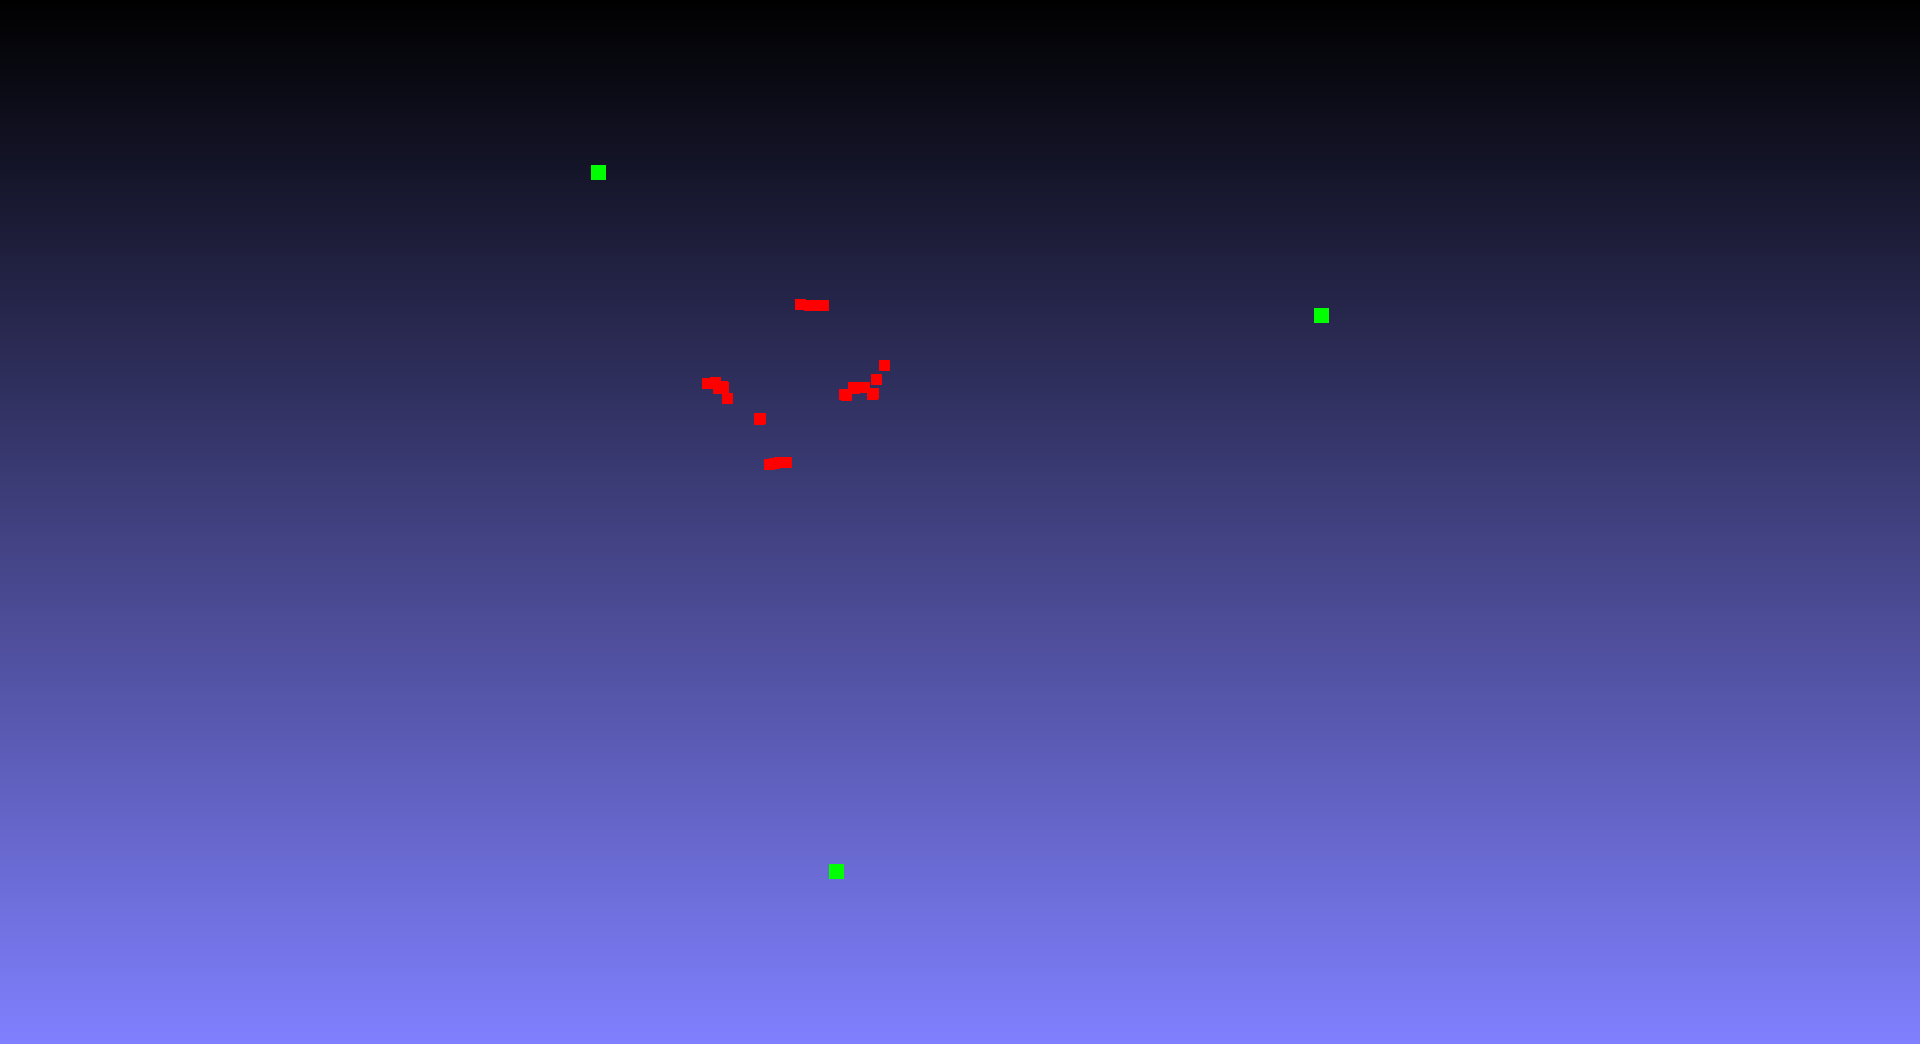
\includegraphics[width=0.5\linewidth]{sfm_filtered}
  \end{tabular}
  \caption{Left to right: (a) The full 3D structure recovered with our
    procudure. (b) Manually filtered 3D structure. Red dots represent scene
    points and green points represent camera locations.}
\end{figure}


\section{Discussion}

The procedure outlined above only work to an extent: When image correspondence
are found reliably between pairs of images. Unfortunately, this is a well known
problem for computer vision algorithms and especially so for uncalibrated
cameras used in this project.

However, as seen in the reconstruction of one of our sample scenes: Evidently
there are a lot of incorrect points but there are also a significant amount of
correct points, as the general structure of the cube is clearly visible despite
limited quality correspondence matching. Thus, it should be possible to re-use
these results in longer pipeline with more elaborate filtering, such as the one
described by \cite{ftc2016}.



\subsection{Future Work}

Computer vision is a very active field with many avenues of research. As such,
there are many ways to improve or tune the algorithm as stated in this work. In
particular, there are many ways one could go about to filter the resulting image
graph that should be able to significantly improve the multi-view correspondence
matching.

Another thing that should be considered in this kind of setup with structured is
the trifocal tensor~\cite{Martyushev_2017}, which should be able to help in
camera setups similar to the ones in this work.

Additionally, this work completely eschewed the use of object detection: In a
larger system, detection of various objects could theoretically be used as a
complement to this kind of system. E.g., if the system detects a person, it is
possible to use a Gaussian approximation of the persons height as a feature
point when estimating the intrinsic camera parameters.

Finally, the system designed during this project is very slow with several
points of synchronization. It would be interesting to see how well this problem,
or a simplified version of it can be parallelized to multi-core systems or GPUs.


\section{Conclusions}



\begin{acks}
\end{acks}

\bibliographystyle{ACM-Reference-Format}
\bibliography{refs}

\end{document}